\chapter{Platforms \& Lifecycles}

\section{Aims}
\paragraph{} At the end of this topic you will be able to:

\begin{itemize}
\item Describe what Android is
\item Describe and use the Android SDK
\item Select and use an IDE
\item Understand the components of an Android App
\item Understand the Activity life-cycle
\end{itemize}

\section{Introducing Android} 
\paragraph{} As you can see we have lots of options for how to develop software for mobile devices. For the practical part of this module, we are going to use Android.

\begin{framed}
\begin{quote}
Android is Google's operating system for mobile devices based on ARM architecture. It is a competitor to the Symbian platform, Apple's iOS for the iPhone and Microsoft's Windows Mobile and Windows Phone for mobile devices all based on ARM architecture.
Android sits on a modified Linux kernel and includes middleware which allow you access to the hardware and key applications. It lets you develop Java but, as with applets on the web, there are some constraints and a philosophical framework.
The Android operating system software stack consists of Java applications running on a Java based object oriented application framework on top of Java core libraries running on a Dalvik virtual machine featuring JIT compilation. … The Android operating system consists of 12 million lines of code including 3 million lines ofXML, 2.8 million lines of C, and 2.1 million lines of Java
\end{quote}

{\begin{flushright}Source: Wikipedia\\\url{http://en.wikipedia.org/wiki/Android_(operating_system)}\end{flushright}}
\end{framed}

\paragraph{} Android was launched by Google/Open Handset Alliance in November 2007 with a competition for developers to design and build prize winning apps – they offered \$1m in prize money. This kick started the Android marketplace. One of the winning apps was an automatic taxi ordering service which read your location in New York and with a single button press ordered a taxi to pick you up; perhaps reason enough to buy a phone?\footnote{See more winners at \url{http://code.google.com/android/adc/gallery_winners.html}}


\section{Development Tools}
\subsection{The SDK}
\paragraph{} The Android SDK is the core set of tools that the Android project have released so that we can develop our own Android apps. The SDK is a mix of tools, that work primarily from the command line, and libraries, which your code can hook into to make use of Android platform features. Whilst the tools work from the command line, there is additional software that you can use to provide graphical user interfaces to the Android tools. For example, Android Studio is an Integrated Development Environments (IDE) which provide a graphical development environment to the command line tools of the SDK. You can build Android apps using only the SDK, however many developers feel more comfortable using an IDE.

\subsection{Development Environments}
\paragraph{} Since December 2014 when version 1.0 was released, the main IDE for Android development has been Android Studio. Prior to this the main IDE was Eclipse, a popular Java development IDE with additional plugins to support Android development. 

\subsection{The Android Debug Bridge}
\paragraph{} Because Android apps are designed and built to run on devices using the Android OS, and not your desktop OS such as Linux, Mac OS, or Windows, you need to provide a way for any apps that you produce to run so that you can test them. For this you have a few options, but you must do at least one of these if you want to be able to run your Android app (and determine that it runs correctly):

\begin{enumerate}
\item The Android Emulator/Android Virtual Device (AVD) - Your IDE provides tools that allow you to run a program that emulates an Android device. In Studio these can be found under Tools $>$ Android $>$ AVD Manager. AVD stands for Android Virtual Device which is the emulated version of the Android OS. Use the AVD Manager to create new devices with various hardware capabilities and software levels. However you should note that emulation is very very very slow. In particular on lab machines, which are running the emulation across the network, you must create AVDs which are very conservative in their hardware, e.g. use lower amounts of RAM, 256MB should be sufficient for most lab practicals, and which use a smaller screensize, e.g. 
\item Hardware - If you have an Android device then you can enable the USB Debugging mode, plug it into your development machine, and it should appear as a connected device which you can select as a target to run your app on. This mode is hidden in a different place on different Android devices so you might have to do a web search for your ``device name+model+enable USB debugging mode''. On OS X and Linux this should 'just work'. On Windows you may have to install drivers for your mobile device before it can be recognised and used to debug Android apps.
\item Virtual Machine - Genymotion\footnote{\url{https://www.genymotion.com/}} is probably the best third party solution for faster virtual Android devices. Underneath it uses the VirtualBox virtualisation software and is much faster than the AVD approach.
\end{enumerate}


\section{Architecture of the Android Platform}
 
\begin{figure}[htb]
\centering
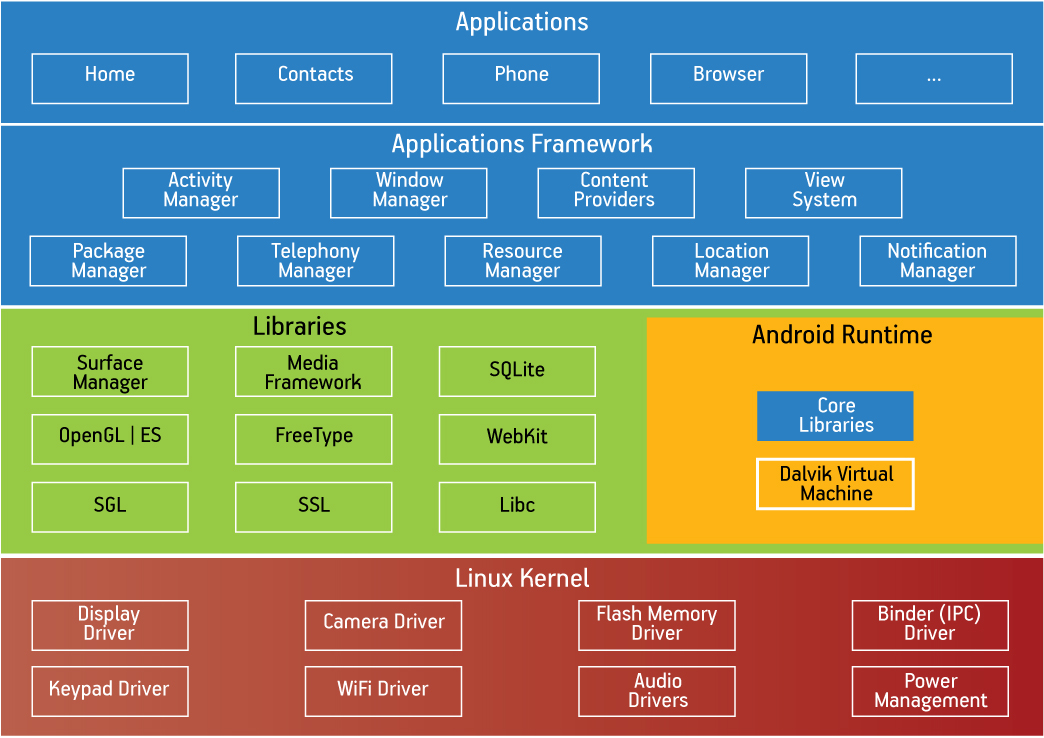
\includegraphics[width=\textwidth]{images/architecture-android}
\caption{The architecture of the Android platform}
\label{fig:architecture-android}
\end{figure}

\section{The Components of apps}
\paragraph{} Android has been designed to let developers take advantage of all the hardware nestling inside your phone. It does this through activities which “do stuff”, services which “do background stuff”,  reusing another app’s functionality (if granted permission) and publishing functionality. Specifically an application is made up of components and a messaging service to communicate between them:

\subsection{Activities}
Think of as a single view or window and one per screen – you can move pages by launching another activity. User interface components are called Views and include scroll-bars, text strings etc (similar to swing components in Java or controls in VS).

\subsection{Services}
A service doesn't have a visual user interface. They run in the background. For example, a service might play background music. Each service extends the Service base class.

\subsection{Broadcast Receivers}
A broadcast receiver is a component that responds to system-wide announcements, for example, that the music player has been switched on, that the battery is low. Your app can also broadcast some information for other apps running on the phone – and interested apps can, as BroadcastReceivers, receive the message (eg change of timezone) and apps can also be BroacastReceivers by extending the BroadcastReceiver base class. You might want to notify the user - through the NotificationManager. These notifications appear on the status bar.

\subsection{Content Provider}
A wrapper for databases and files, the content provider can make app data available to other apps

\section{The Activity Lifecycle}


\begin{figure}[htb]
\centering
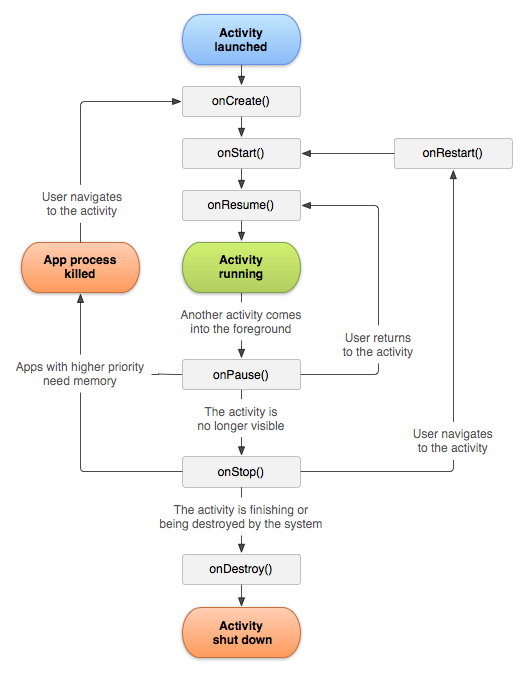
\includegraphics[width=0.8\textwidth]{images/android_lifecycle_original}
\caption{The lifecycle of Android activities.}
\label{fig:lifecycle-android-activities}
\end{figure}


\begin{figure}[htb]
\centering
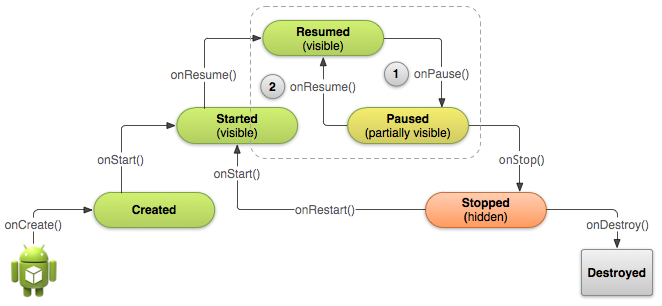
\includegraphics[width=\textwidth]{images/android_lifecycle_state-diagram}
\caption{A slightly re-arranged diagram of the lifecycle of Android activities.}
\label{fig:lifecycle-android-activities-state-diargram}
\end{figure}



\paragraph{} Activities and services are activated by intents. Intents are asynchronous messages used by the OS to match task requests with activities and services. The Intent object is a bundle of information: it ``contains information of interest to the component that receives the intent (such as the action to be taken and the data to act on) plus information of interest to the Android system (such as the category of component that should handle the intent and instructions on how to launch a target activity)''\footnote{\url{http://developer.android.com/guide/topics/intents/intents-filters.html}}.


\paragraph{} Instead of a main method defining where things kick off, you must define a class which extends (or inherits from) Activity. An Activity class simply means that it can run and do stuff.
The onCreate() method will be called when your Activity starts — it is where you should perform all initialization and UI setup. The onCreate() method will be called by the Android system when your Activity starts — it is where you should perform all initialization and UI setup. [The @Override statement is a Java convention - it simply flags up your intention to override a method in the superclass so the compiler can check that’s what you actually end up doing – and flag it if that’s not what the net effect is.] The Bundle is a mechanism for living with the complexity of multiple activities, multiple entry points etc. The bundle refers to the data required to run your activity effectively – eg what is the current state of your activity, have you been interrupted by a phone call for example.
A View is a drawable object eg button, image or, in this case, some text. TextView is a subclass of view. We construct a TextView object (tv). The constructor parameter this refers to is an Android Context. A Context is a handle to the system – providing preferences, access to databases etc. The Activity class inherits from the Context so this is a context.  
The app then calls the setText() method of the tv object.
Finally, you pass the tv to setContentView() in order to display it as the content for the Activity UI. If your Activity doesn't call this method, then no UI is present and the system will display a blank screen.




\section{Summary}
\paragraph{} In this topic we have learnt to:

\begin{itemize}
\item Describe what Android is
\item Describe and use the Android SDK
\item Select and use an IDE
\item Understand the components of an Android App
\item Understand the Activity life-cycle
\end{itemize}


%\section{Directed Study}
%\paragraph{}

%\section{References \& Resources}

